\section{Présentation}
\ifprof
\else
L’Intelligence Artificielle est de plus en plus utilisée dans de nombreux domaines divers et variés.
Les techniques d’apprentissage machine, qui permettent à un logiciel d’apprendre automatiquement à
partir de données au lieu d’être explicitement programmé, fournissent des résultats impressionnants.
Les applications sont nombreuses dans la reconnaissance d’image, la compréhension de la parole ou
de textes, dans l’assistance à la décision, dans la classification de données, dans la robotique...
L’Intelligence Artificielle progresse également dans le domaine de la santé. Le logiciel Watson développé
par IBM peut analyser les données d’un patient : ses symptômes, ses consultations médicales,
ses antécédents familiaux, ses données comportementales, ses résultats d’examen, etc. Il établit alors
une prévision de diagnostic le plus vraisemblable et propose des options de traitement en s’appuyant
sur une base de données établie sur un grand nombre de patients.

\begin{obj}
L’objectif du travail proposé est de découvrir quelques techniques d’Intelligence Artificielle en
s’appuyant sur un problème médical. À partir d’une base de données comportant des propriétés
sur le bassin et le rachis lombaire (figures 1), on cherche à déterminer si un patient peut être
considéré comme « normal » ou bien si ces données impliquent un développement anormal de
type hernie discale (saillie d’un disque intervétébral) ou spondylolisthésis (glissement du corps
vertébral par rapport à la vertèbre sous-jacente).
\end{obj}

\begin{center}
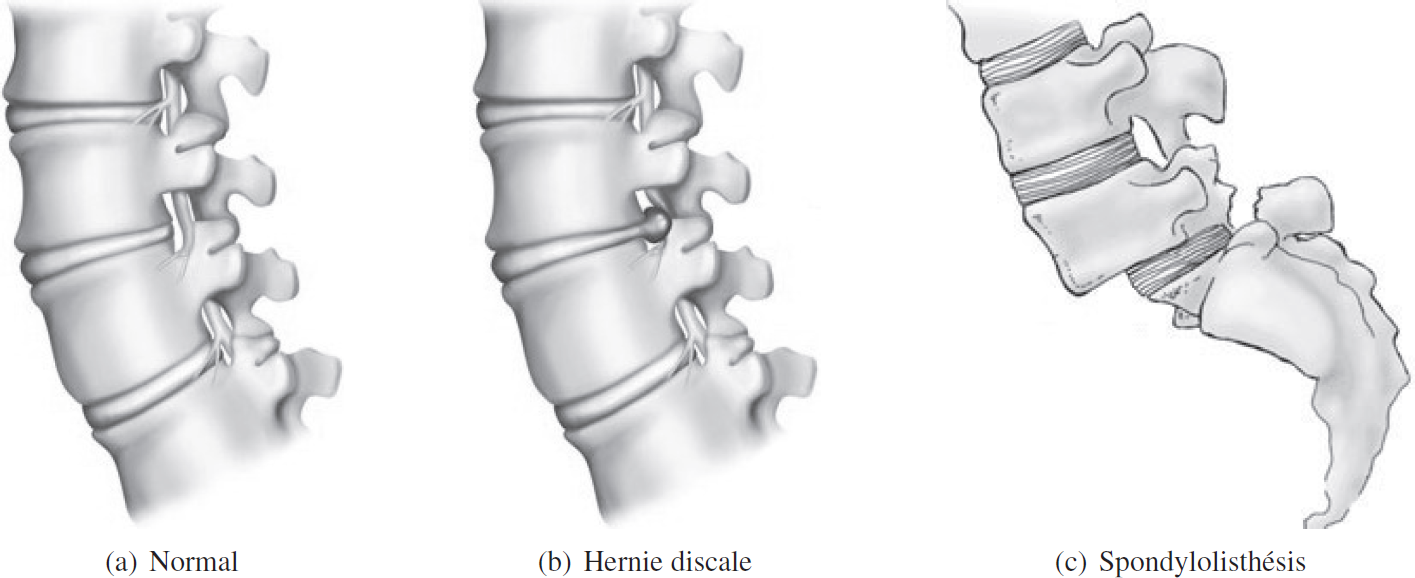
\includegraphics[width=.8\textwidth]{images/fig_01}

Figure 1 -- Différentes configurations des vertèbres
\end{center}

Le sujet abordera les points suivants :
\begin{itemize}
\item analyse et représentation des données;
\item prédiction à l’aide de la méthode \textit{k}-NN;
\item apprentissage et prédiction à l’aide de la méthode dite « Naïve Bayes ».
\end{itemize}

Dans tout le sujet, il sera supposé que les modules python \texttt{numpy}, \texttt{matplotlib.pyplot} sont déjà
importés dans le programme.
\fi
\section{Analyse des données}
\ifprof
\else
La base de données médicale contient des informations administratives sur les patients et des informations
médicales. Pour simplifier le problème, on considère deux tables : PATIENT et MEDICAL.

\begin{minipage}[c]{.5\linewidth}
La table PATIENT contient les attributs suivants :
\begin{itemize}
\item id : identifiant d’un individu (entier), clé primaire ;
\item nom : nom du patient (chaîne de caractères) ;
\item prenom : prénom du patient (chaîne de caractères) ;
\item adresse : adresse du patient (chaîne de caractères) ;
\item email : (chaîne de caractères) ;
\item naissance : année de naissance (entier).
\end{itemize}
\end{minipage} \hfill
\begin{minipage}[c]{.45\linewidth}
\begin{center}
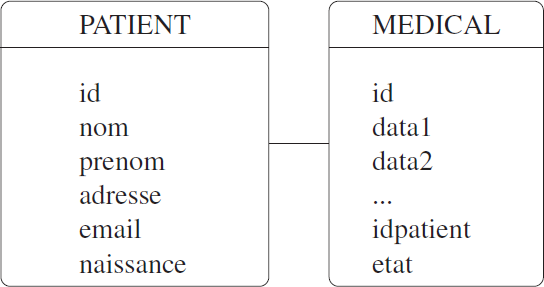
\includegraphics[width=.85\linewidth]{images/fig_a}
\end{center}
\end{minipage} 

La table MEDICAL contient les attributs suivants :
\begin{itemize}
\item id : identifiant d’un ensemble de propriétés médicales (entier), clé primaire ;
\item data1 : donnée (flottant) ;
\item data2 : donnée (flottant) ;
\item ... ;
\item idpatient : identifiant du patient représenté par l’attribut id de la table PATIENT (entier) ;
\item etat : description de l’état du patient (chaîne de caractères).
\end{itemize}

Les attributs data1, data2... sont des données relatives à l’analyse médicale souhaitée (dans notre cas
des données biomécaniques). L’attribut «~etat~» permet d’affecter un label à un ensemble de données
médicales : «~normal~», «~hernie discale~», «~spondylolisthésis~».
\fi

\subparagraph{}\textit{Écrire une requête SQL permettant d’extraire les identifiants des patients ayant une «~hernie
discale~».}

\ifprof
\begin{corrige}
\texttt{SELECT idpatient FROM MEDICAL WHERE etat=''hernie discale'';}
\end{corrige}
\else
\fi

\subparagraph{}\textit{Écrire une requête SQL permettant d’extraire les noms et prénoms des patients atteints de
« spondylolisthésis ».}
\ifprof
\begin{corrige} ~\\
\texttt{SELECT nom, prenom FROM PATIENT}

					\texttt{JOIN MEDICAL}
					
					\texttt{ON PATIENT.id = MEDICAL.idpatient}
					
					\texttt{WHERE MEDICAL.etat=''spondylolisthésis'';}
\end{corrige}
\else
\fi

\subparagraph{}\textit{Écrire une requête SQL permettant d’extraire chaque état et le nombre de patients pour chaque
état.}
\ifprof
\begin{corrige}
~\\
\texttt{SELECT etat, COUNT(DISTINCT idpatient) FROM MEDICAL}

					\texttt{GROUP BY etat}
					
\end{corrige}
\else
\fi

\ifprof
\else
Une telle base de données permet donc de faire de nombreuses recherches intéressantes pour essayer
de trouver des liens entre les données des patients et une maladie. Cependant, compte-tenu du nombre
d’informations disponibles, il est nécessaire de mettre en place des outils pour aider à la classification
de nouveaux patients. C’est l’objet des algorithmes d’Intelligence Artificielle développés dans la suite.
Pour l’étude qui va suivre, on extrait de la base de données les attributs biomécaniques de chaque
patient que l’on stocke dans un tableau de réels (codés sur 32 bits) à $N$ lignes (nombre de patients)
et $n$ colonnes (nombre d’attributs égal à 6 dans notre exemple). On nomme \texttt{data} ce tableau. L’état
de santé est stocké dans un vecteur de taille $N$ contenant des valeurs entières (codées sur 8 bits)
correspondant aux différents états pris en compte (0 : normal, 1 : hernie discale, 2 : spondylolisthésis).
On le nomme : \texttt{etat}.

Les variables \texttt{data} et \texttt{etat} sont stockées dans des objets de type \texttt{array} de la bibliothèque Numpy.
Des rappels quant à l’utilisation de ce module Python sont donnés dans l’annexe.
\fi

\subparagraph{}\textit{Citer un intérêt d’utiliser la bibliothèque de calcul numérique Numpy quand les tableaux sont
de grande taille.}
\ifprof
\begin{corrige}
Les tableaux Numpy ont une taille fixe dans l'espace mémoire. Cela doit permettre de réduire l'espace utilisé et les temps de calcul. 
\end{corrige}
\else
\fi

\subparagraph{}\textit{Déterminer la quantité de mémoire totale en Mo ( $\SI{1}{Mo} = \SI{1 000 000}{octets}$) nécessaire pour stocker le tableau et le vecteur des données si $N = \num{100 000}$. On supposera que les données
sont représentées en suivant la norme usuelle IEEE 754.}
\ifprof
\begin{corrige} ~\\

La taille prise par le tableau \texttt{data} est $\num{100000} \times 6 \times 32/8=\SI{2,4}{Mo}$. 

La taille prise par le vecteur \texttt{etat} est $\num{100000} \times 1=\SI{0,1}{Mo}$.
\end{corrige}
\else
\fi

\ifprof
\else
Les 6 attributs considérés dans notre exemple (les n colonnes du tableau) sont définis ci-après :
\begin{itemize}
\item angle d’incidence du bassin en \degres ;
\item angle d’orientation du bassin en \degres ;
\item angle de lordose lombaire en \degres ;
\item pente du sacrum en \degres ;
\item rayon du bassin en mm;
\item distance algébrique de glissement de spondylolisthésis en mm.
\end{itemize}

Les labels de ces attributs sont stockés dans une liste nommée :
\texttt{label\_attributs = [‘incidence\_bassin’, ‘orientation\_bassin’, ‘angle\_lordose’,
‘pente\_sacrum’, ‘rayon\_bassin’, ‘glissement\_spon’]}.
Le tableau suivant montre les premières valeurs du tableau \texttt{data}.

\footnotesize
\begin{center}
\begin{tabular}{|c|c|c|c|c|c|}
\hline
incidence\_bassin & orientation\_bassin & angle\_lordose & pente\_sacrum & rayon\_bassin & glissement\_spon \\ \hline
63,03&	22,55& 	39,61& 	40,48& 	98,67& 	-0,25\\ \hline
39,06& 	10,06& 	25,02& 	29,0&	114,41& 	4,56\\ \hline
68,83& 	22,22& 	50,09& 	46,61& 	105,99& 	-3,53\\ \hline
69,3& 	24,65& 	44,31& 	44,64& 	101,87& 	11,21\\ \hline
49,71& 	9,65& 	28,32& 	40,06& 	108,17& 	7,92  \\ \hline
40,25& 	13,92&	25,12& 	26,33& 	130,33& 	2,23  \\ \hline
48,26& 	16,42& 	36,33& 	31,84& 	94,88& 	28,34 \\ \hline
\end{tabular}
\end{center}
\normalsize 
\begin{center}
Tableau 1 -- Données (partielles) des patients à diagnostiquer
\end{center}


Avant de traiter les données pour réaliser une prédiction (ou diagnostic), il peut être intéressant de
les visualiser en traçant un attribut en fonction d’un autre attribut et en utilisant des motifs différents
selon les valeurs du vecteur \texttt{etat}.
On obtient, à partir des données exploitées, les courbes de la figure 2 (zoom sur la figure 3).



\begin{center}
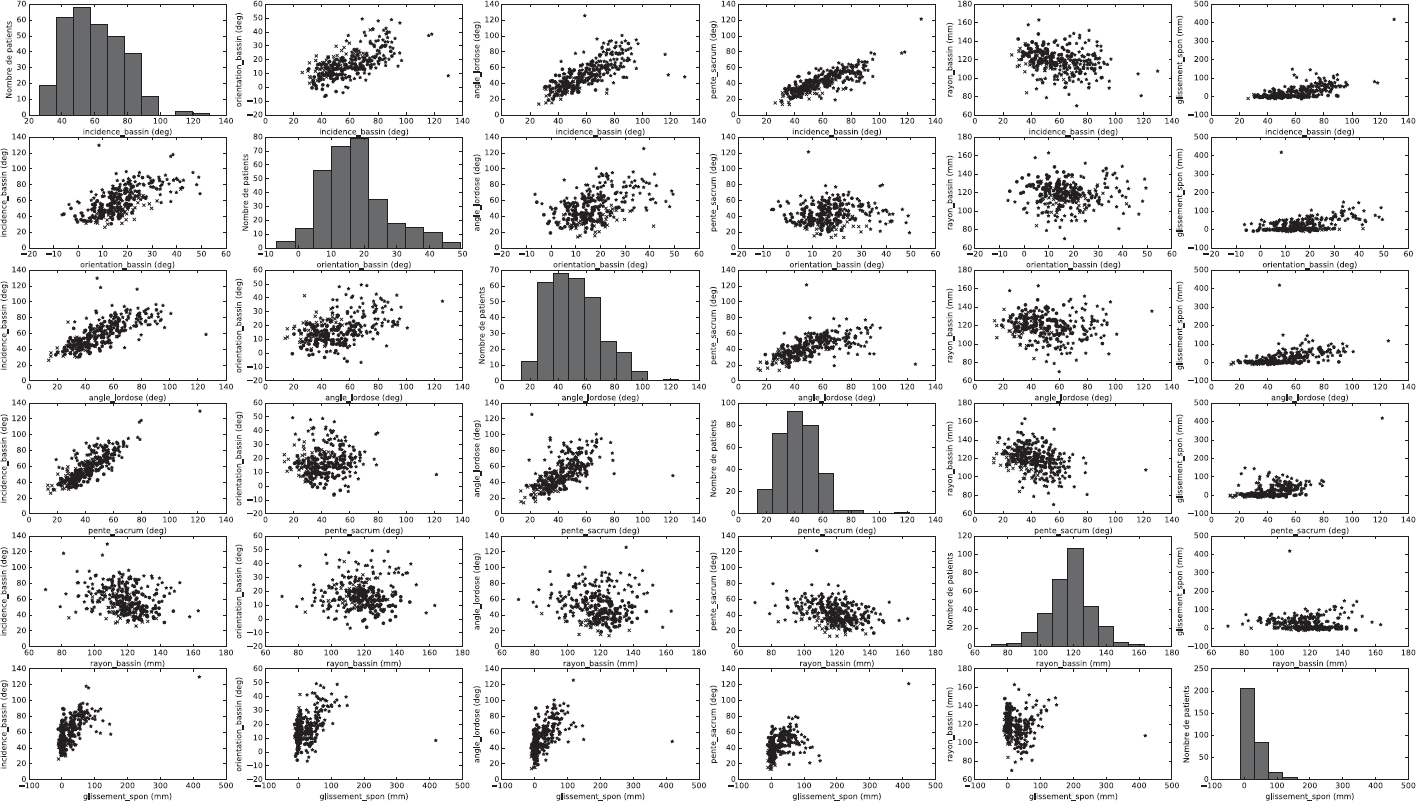
\includegraphics[width=\textwidth]{images/fig_02}
Figure 2 -- Répartition des données
\end{center}


\begin{center}
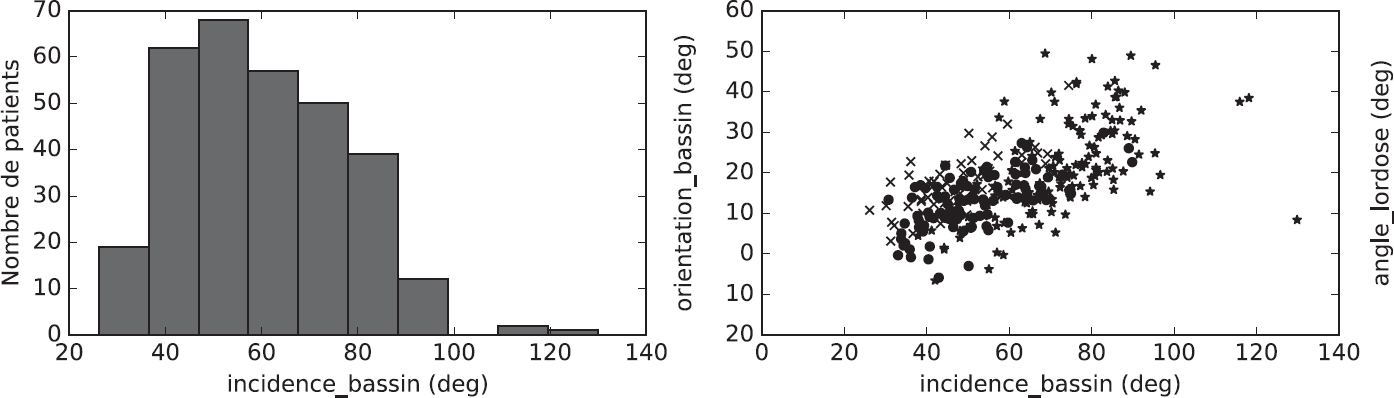
\includegraphics[width=.8\textwidth]{images/fig_03}

Figure 3 -- Zoom sur les figures de coordonnées (1,1) et (1,2) de la matrice de répartition des données
(figure 2)
\end{center}


Cette figure est une matrice dont le terme $(i, i)$ de la diagonale est l’histogramme des fréquences de
l’attribut $i$ et les termes extra-diagonaux $(i, j)$ représentent l’attribut $i$ en fonction de l’attribut $j$ pour
chaque ligne du tableau \texttt{data}.

Sur les figures hors diagonale, on représente chaque donnée d’attribut $i$ en fonction de l’attribut $j$ à
l’aide d’un symbole dépendant de l’état du patient (un rond ’o’ si l’état du patient est normal, une
croix ’x’ si l’état est <<~hernie discale~>> et une étoile ’*’ si l’état est <<~spondylolisthésis~>>).
Pour réaliser cette figure, il faut séparer les données en fonction de l’état du patient afin d’affecter un
symbole par état. Ceci revient à classer les patients en plusieurs groupes.

\fi

\subparagraph{}\textit{Écrire une fonction \pyv{separationParGroupe(data,etat)} qui sépare le tableau data en
3 sous-tableaux en fonction des valeurs du vecteur etat correspondantes (on rappelle que
celui-ci contient les valeurs 0, 1 et 2 uniquement). La fonction doit renvoyer une liste de
taille 3 de sous-tableaux. Les sous-tableaux ne seront pas nécessairement représentés par un
type ’array’; ’liste de listes’, ’liste d’array’ conviennent également.}
\ifprof
\begin{corrige}
Le tableau data est de la forme [[0,1,2,3,4,5],[6,7,8,9,10,11],...]
\begin{lstlisting}[language=Python]
def separationParGroupe(data,etat) :
    N = len(etat)
    normal = []
    hernie  = []
    spondy = []
    for i in range(N) :
        if etat[i] == 1 :
            normal.append(data[i])
        elif etat[i] == 2 :
            hernie.append(data[i])
        elif etat[i] == 3 :
        	spondy.append(data[i])
    return normal, hernie, spondy
\end{lstlisting}

Autre possibilité : 
\begin{lstlisting}[language=Python]
def separationParGroupe(data,etat) :
    return [[data[i] for i in range(len(data)) if etat[i]==j] for j in range(3)]
\end{lstlisting}

\end{corrige}
\else
\fi


\ifprof
\else
Pour définir la figure, les instructions suivantes sont exécutées :


\begin{lstlisting}[language=Python]
fig = plt.figure()
mark = ["o","x","*"]
label_attributs = ["incidence_bassin(deg)","orientation_bassin(deg)",
				"angle_lordose(deg)", "pente_sacrum(deg)",
				"rayon_bassin(mm)", "glissement_spon (mm)"]
groupes = separationParGroupe (data, etat)
for i in range (len(groupes)):
    groupes[i] = array(groupes[i])

n=len(data[0])
for i in range(n) :
    for j in range(n) :
        ax1 = plt.subplot(ARGS1)
        plt.ylabel(label_attributs[j]) # mettre un label a l'axe y
        if TEST :
            for k in range (len(groupes)) :
                plt.xlabel(label_attributs[i]) # mettre un label a l'axe x
                ax1.scatter(ARGS2)
        else :
            plt.xlabel("Nombre de patients") # mettre un label a l'axe x
            ax1.hist(ARGS3)
plt.show()
\end{lstlisting}

Les instructions précédentes utilisent la fonction \pyv{separationParGroupe} définie à la question Q6,
puis les éléments de la liste groupes sont convertis en array afin de pouvoir extraire les colonnes
plus facilement.

La documentation du module matplotlib (plt) renseigne sur les arguments des fonctions subplot,
scatter et hist.



\begin{lstlisting}[language=Python]
ax1 = plt.subplot(a, b, k)
\end{lstlisting}

Cette instruction permet de sélectionner parmi un tableau de figures de taille $a$ (nombre de lignes),
$b$ (nombre de colonnes), la $k$\ieme \~ en numérotant les sous-figures de 1 à $m \times n$ en partant du haut gauche
vers le bas droite (en allant de gauche à droite et de haut en bas).

\begin{lstlisting}[language=Python]
ax1.scatter(datax, datay, marker=mark[k])
\end{lstlisting}

Cette commande permet de tracer sur la sous-figure ax 1 un nuage de points d’abscisses un vecteur
\texttt{datax} et d’ordonnées un vecteur \texttt{datay} avec un symbole à choisir parmi ceux de la liste \texttt{mark}.

\begin{lstlisting}[language=Python]
ax1.hist(datax)
\end{lstlisting}

Cette commande permet de tracer un histogramme des données \texttt{datax} sur la sous-figure ax 1.

\fi

\subparagraph{}\textit{Définir les arguments ARGS1, ARGS2, ARGS3 ainsi que la condition TEST définis dans le
script précédent permettant d’obtenir la figure 2.}
\ifprof
\begin{corrige}
\begin{lstlisting}[language=Python]
ax1 = plt. subplot ( n, n, i*n+j+1)
ax1.scatter(groupes [k][:,i], groupes[k][:,j], marker=mark[k])
ax1.hist(data[:,j])

# Test
if i != j:
\end{lstlisting}
\end{corrige}
\else
\fi

\subparagraph{}\textit{Préciser l’utilité des diagrammes de la diagonale ainsi que celle des diagrammes hors diagonale.}
\ifprof
\begin{corrige}
Les diagrammes sur la diagonale donnent la répartition des patients en fonction de l’attribut $j$.
Les autres diagrammes donnent un attribut en fonction d’un autre, ils permettent de
voir s’il y a un lien de corrélation entre 2 attributs. De plus ils permettent de visualiser
les répartitions de ces attributs en fonction de l’état de l’individu.
\end{corrige}
\else
\fi


\section{Apprentissage et prédiction}

\subsection{Méthode \textit{k}-NN}
\ifprof
\else
La méthode \textit{k}-NN est une méthode d’apprentissage dite supervisée; les données sont déjà classées par
groupes clairement identifiés et on cherche dans quels groupes appartiennent de nouvelles données.
Le principe de la méthode est simple. Après avoir calculé la distance euclidienne entre toutes les
données connues des patients et les données d’un nouveau patient à classer, on extrait les K données
connues les plus proches. L’appartenance du nouveau patient à un groupe est obtenue en cherchant le
groupe majoritaire, c’est-à-dire, le groupe qui apparaît être le plus représentatif parmi les K données
connues.

On note $X_i$, $i \in \llbracket 0,n-1 \rrbracket $, le vecteur colonne $i$ du tableau de données data, c’est-à-dire les valeurs
prises par l’attribut $i$ des données des patients déjà classées. On cherche à déterminer à quel groupe
appartient un nouveau patient dont les attributs sont représentés par un n-uplet $z$ de valeurs notées
$\left(z_0, z_1, ..., z_{n-1} \right)$.
\fi
\subsection*{Préparation des données}

\ifprof
\else
Avant de calculer la distance euclidienne, il est préférable de normaliser les attributs pour éviter qu’un
attribut ait plus de poids par rapport à un autre. On choisit de ramener toutes les valeurs des attributs
entre 0 et 1.

Une technique de normalisation consiste à rechercher pour chaque attribut $X$ le minimum ($\min(X)$)
qui est placé à 0 et le maximum ($\max(X)$) qui est placé à 1. On note alors $X_{\text{norm}}$ un des vecteurs
colonne $X$ après normalisation (toutes les valeurs de $X_{\text{norm}}$ sont donc comprises entre 0 et 1).
\fi

\subparagraph{}\textit{Proposer une expression de $x_{\text{normj}}$ un élément du vecteur $X_{\text{norm}}$ en fonction de l’élément $x_j$ du
vecteur $X$ correspondant et de $\min(X)$ et $\max(X)$.}
\ifprof
\begin{corrige}
En utilisant une correction linéaire où les $x_j$ sont << étalés >> entre 0 et 1, on a 
$x_{\text{normj}} =a x_j + b $ avec $x_{\text{normj}}=0$ pour $x_j =\min(X)$ et  $x_{\text{normj}}=1$ pour $x_j =\max(X)$. 

On a donc $0 =a\min(X)+ b $ et $1 =a \max(X) + b $ soit $b =-a\min(X) $ et $1 =a \left(\max(X)-\min(X)\right) $ $\Leftrightarrow a= \dfrac{1}{\max(X)-\min(X)} $. On a donc $b =-\dfrac{\min(X)}{\max(X)-\min(X)} $.


Par suite, $x_{\text{normj}} = \dfrac{1}{\max(X)-\min(X)} x_j -\dfrac{\min(X)}{\max(X)-\min(X)}$.

Au final,  $x_{\text{normj}} = \dfrac{ x_j -\min(X)}{\max(X)-\min(X)}$.
\end{corrige}
\else
\fi

\subparagraph{}\textit{Écrire une fonction \pyv{min_max(X)} qui retourne les valeurs du minimum et du maximum d’un vecteur X passé en argument. La fonction devra être de complexité linéaire.}
\ifprof
\begin{corrige}
\begin{lstlisting}[language=Python]
def min_max(X):
    mini = X[0]
    maxi = X[0]
    N = len(X)
    for i in range (N):
        if X[i]<mini :
            min = X[i]
        if X[i]>maxi :
            maxi = X[i]
    return min,max
\end{lstlisting}
\end{corrige}
\else
\fi

\subparagraph{}\textit{Écrire une fonction \pyv{distance(z,data)} qui parcourt les N lignes du tableau data et calcule
les distances euclidiennes entre le $n$-uplet $z$ et chaque $n$-uplet $x$ du tableau de données connues
(x représente une ligne du tableau). La fonction doit renvoyer une liste de taille $N$ contenant
les distances entre chaque $n$-uplet $x$ et le $n$-uplet $z$.}
\ifprof
\begin{corrige}
On considère que le valeurs de data ont été normalisées.

\begin{lstlisting}[language=Python]
def distance(z,data):
    res = []
    for X in data :
        d = 0
        for i in range(len(z)):
            d=d+(z[i]-X[i])**2
        res = res.append(math.sqrt(d))
    return res
\end{lstlisting}

\end{corrige}
\else
\fi

\subsection*{Détermination des $k$ plus proches voisins}

\ifprof
\else
Pour déterminer les $k$ plus proches voisins avec $k$ un entier choisi arbitrairement, il suffit d’utiliser
un algorithme de tri efficace. La liste T à trier est une liste de listes à 2 éléments contenant :
\begin{itemize}
\item la distance entre le $n$-uplet à classer et un $n$-uplet connu (on trie par ordre croissant sur ces
valeurs) ;
\item la valeur de l’état correspondant au $n$-uplet connu.
\end{itemize}

On admet que la fonction \pyv{tri(T)} trie en place la liste \pyv{T}.
%On retient l’algorithme suivant :
%
%\begin{lstlisting}[language=Python]
%01. def tri(T) :
%02.     if len(T) <= 1 :
%03.         return T
%04.     else :
%05.         m= len(T) // 2
%06.         tmp1 = [ ]
%07.         for x in range (m) :
%08.             tmp1.append (T[x])
%09.         tmp2 = [ ]
%10.         for x in range (m, len(T)) :
%11.             tmp2.append(T[x])
%12.         return fct(tri(tmp1), tri(tmp2))
%13. 
%14. def fct(T1,T2) :
%15.     if T1 == [ ] :
%16.         . . . . . . . . . . . . . . . . . . . # ligne 1 a compléter
%17.     if T2 == [ ] :
%18.         . . . . . . . . . . . . . . . . . . . # ligne 2 a compléter
%19.     if T1[0][0] < T2[0][0] :
%20.         return [T1[0]]+fct(T1[1:],T2)
%21.     else :
%22.          . . . . . . . . . . . . . . . . . . . # ligne 3 a compléter
%\end{lstlisting}
%
%\subparagraph{}\textit{Donner le nom de ce tri ainsi que son intérêt par rapport à un tri par insertion. Préciser un inconvénient du programme proposé par rapport à ce tri.}
%
%\subparagraph{}\textit{Préciser les lignes 1 à 3 de la fonction \pyv{fct} pour que l’algorithme de tri soit fonctionnel.}

L’algorithme de la méthode KNN est décrit par la fonction python suivante :
\begin{lstlisting}[language=Python]
01. def KNN(data, etat, z, K, nb) :
02.    # partie1
03.    T= []
04.    dist = distance (z, data)
05.    for i in range (len(dist)) :
06.        T.append([dist[i],i])
07.    tri(T)
08.
09.    # partie 2
10.    select = [0]*nb
11.    for i in range (K) :
12.        select[etat[T[i][1]]]+=1
13.
14.    # partie 3
15.    ind = 0
16.    res = select [0]
17.    for k in range(1, nb) :
18.        if select[k] > res :
19.            res = select[k]
20.           ind = k
21.    return ind
\end{lstlisting}

$K$ représente le nombre de voisins proches retenus, $nb$ correspond au nombre d’état (3 dans notre
exemple) et $z$ correspond aux attributs du patient à classer.

\fi

\subparagraph{}\textit{Expliquer ce que font globalement les parties 1 (lignes 3 à 7), 2 (lignes 10 à 12) et 3 (lignes 15
à 21) de l’algorithme. Préciser ce que représentent les variables locales T, dist, select, ind.}
\ifprof
\begin{corrige}
Les lignes 3 à 7 permettent, pour un individu $z$, de lui associer la distance d'un individu contenu dans data et de lui associé l'état de l'individu. 
Cette liste est alors triée en fonction des distances. Les $k$ premiers individus de $T$ sont donc les $k$ individus les plus proches de $z$.

La partie 2 permet de compter, parmi les $k$ plus proches voisins de $z$, le nombre d'individus par état.

La partie 3 permet de déterminer dans quel état est probablement l'individu $z$.

De fait, on a :
\begin{itemize}
\item T : liste triée contenant des couples (distance, état);
\item dist : liste des distances entre $z$ et data;
\item select : select[i] est le nombre de patient à l'état i parmi les $k$ plus proches voisins;
\item ind :représente l'indice i où select[i] est le plus grand.
\end{itemize}
\end{corrige}
\else
\fi

\subsection*{Validation de l’algorithme}

\ifprof
\else

Pour tester l’algorithme, on utilise un jeu de données supplémentaires normalisées dont l’état des
patients est connu (100 patients). On note \pyv{datatest} ces données et \pyv{etattest} le vecteur d’état connu
pour ces patients. On applique ensuite l’algorithme sur chaque élément de ce jeu de données pour une
valeur de $k$ fixée.

On définit la fonction suivante qui renvoie une matrice appelée <<~matrice de confusion~>>.

\begin{lstlisting}[language=Python]
def test_KNN (datatest, etattest, data, etat, K, nb) :
    etatpredit = []
    for i in range (len(datatest)) :
        res = KNN(data, etat, datatest[i], K, nb)
        etatpredit.append(res)

    mat = np.zeros((nb, nb))
    for i in range(len(etattest)) :
        mat[etattest[i], etatpredit[i]]+=1
    return mat
\end{lstlisting}

On obtient pour $K = 8$ la matrice suivante : $\begin{pmatrix}23 & 4 & 7 \\ 7 & 11 & 1 \\ 5 & 2 & 40 \end{pmatrix}$.

\fi

\subparagraph{}\textit{Indiquer l’information apportée par la diagonale de la matrice. Exploiter les valeurs de la première ligne de cette matrice en expliquant les informations que l’on peut en tirer. Faire de
même avec la première colonne. En déduire à quoi sert cette matrice.}
\ifprof
\begin{corrige}
La diagonale permet de savoir le nombre de patients détectés à l'état $i$ qui sont réellement à l'état $i$.
La première ligne permet de connaître le nombre de patients à l'état 0 qui ont été détectés à l'état 0 (première ligne, première colonne), à l'état 1 (première ligne, deuxième colonne) et à l'état 3 (première ligne, troisième colonne).

On peut tenir le même raisonnement pour la première colonne. Cette matrice permet de détecter les erreurs faites par l'algorithme \textit{k}-NN.
\end{corrige}
\else
\fi

\ifprof
\else
On peut également tracer l’efficacité de l’algorithme pour différentes valeurs de $k$ sur le jeu de données
test (100 éléments sur un échantillon de 310 données). On trace le pourcentage de réussite en
fonction de la valeur de $K$ sur la figure 4.

\begin{center}
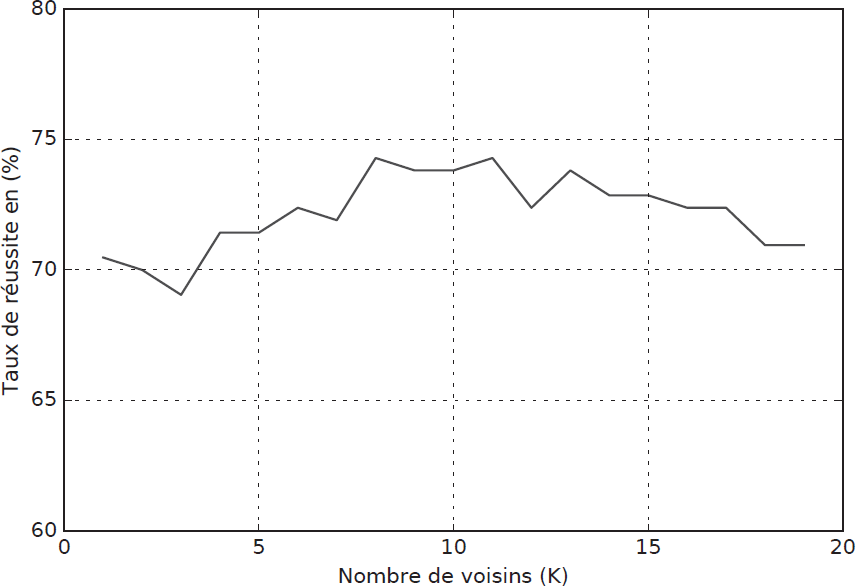
\includegraphics[width=.5\textwidth]{images/fig_04}

Figure 4 -- Pourcentage de réussite de l’algorithme en fonction de $K$
\end{center}
\fi

\subparagraph{}\textit{Commenter la courbe obtenue et critiquer l’efficacité de l’algorithme.}
\ifprof
\begin{corrige}
\begin{itemize}
\item On nombre de voisins compris entre 8 et 11 semble optimal.
\item La détermination de $k$ semble empirique.
\item Plus $k$ est grand, plus l'algorithme est lent.
\end{itemize}
\end{corrige}
\else
\fi

\subsection{Méthode de classification naïve bayésienne}
\ifprof
\else
Une autre méthode simple à mettre en œuvre et qui fournit de bons résultats, malgré l’hypothèse
forte utilisée, est la classification naïve bayésienne. Cette méthode d’apprentissage est supervisée
également. La méthode repose sur le théorème de Bayes qui suppose l’indépendance probabilistique
des caractéristiques d’un groupe donné.

On suppose que chaque attribut $i$ (colonne de la matrice de données data) est modélisable par une
variable aléatoire notée $X_i$ pour $i \in \llbracket 0,n-1 \rrbracket$. L’appartenance d’une donnée à un groupe est modélisée par la variable aléatoire $Y$, dont les valeurs discrètes sont $y_0 = 0$ pour un sujet sain, $y_1 = 1$ pour un
sujet atteint d’une hernie discale et $y_2 = 2$ pour un sujet atteint de spondylolisthésis.

L’appartenance de la donnée $k$ ($k$\ieme \~ ligne de la matrice de données) est connue et indiquée dans le vecteur \pyv{etat}.


Le théorème de Bayes permet de déterminer la probabilité qu’une donnée appartienne à un groupe $y_j$
connaissant ses attributs $x_i$.

$$
P\left(Y=y_j  | X_0 = x_0, X_1 = x_1, ..., X_{n-1} = x_{n-1} \right) 
= \dfrac{P\left(Y = y_j\right) \times  P\left(X_0 = x_0, X_1 = x_1, ..., X_{n-1} = x_{n-1} |Y = y_j\right)}{ P\left(X_0 = x_0, X_1 = x_1, ..., X_{n-1} = x_{n-1} \right)}
$$

où :
\begin{itemize}
\item $P\left(Y=y_j  | X_0 = x_0, X_1 = x_1, ..., X_{n-1} = x_{n-1} \right)$ est la probabilité d’appartenir au groupe yj sachant
que les différentes variables aléatoires Xi prennent respectivement les valeurs xi;
\item $P\left(Y = y_j\right)$ est la probabilité d’appartenir au groupe yj;
\item $P\left(X_0 = x_0, X_1 = x_1, ..., X_{n-1} = x_{n-1} |Y = y_j\right)$ est la probabilité que les différentes variables
aléatoires Xi prennent respectivement les valeurs xi sachant que la donnée appartient au groupe
yj;
\item $P\left(X_0 = x_0, X_1 = x_1, ..., X_{n-1} = x_{n-1} \right)$ est la probabilité que les différentes variables aléatoires Xi prennent respectivement les valeurs xi.
\end{itemize}

L’hypothèse naïve bayésienne suppose que tous les attributs sont indépendants et donc que :
$$P\left(X_0 = x_0, X_1 = x_1, ..., X_{n-1} = x_{n-1} |Y = y_j\right) = \prod\limits_{i} P\left( X_i=x_i | Y=y_j\right).$$



Comme le dénominateur $P\left(X_0 = x_0, X_1 = x_1, ..., X_{n-1} = x_{n-1}\right)$ est indépendant du groupe considéré et donc constant, on ne considère que le numérateur :
$$P\left(Y = y_j\right) \times  P\left(X_0 = x_0, X_1 = x_1, ..., X_{n-1} = x_{n-1} |Y = y_j\right).$$

Pour déterminer le groupe le plus probable auquel appartient une donnée $z$ à classer, représentée par
le $n$-uplet $(z_0, z_1, ..., z_{n-1})$, on choisit la probabilité maximale $P\left(Y = y_j\right) \times \prod\limits_{i}P\left(X_i=z_i | Y=y_j\right)$  parmi
les $j$ groupes.

Des lois de probabilités diverses sont utilisées pour estimer $P\left(X_i = z_i|Y = y_j\right)$; nous utiliserons une loi de distribution gaussienne.

\fi

\subsection*{Apprentissage}

\ifprof
\else
La première étape consiste à séparer les données selon les groupes auxquels elles appartiennent. On
réutilise pour cela la fonction \pyv{separationParGroupe(data,etat)} définie à la question Q6.


Pour calculer la probabilité conditionnelle $P\left(X_i = z_i|Y = y_j\right)$ d’une donnée $z$ représentée par le $n$-uplet $\left(z_0, z_1, ..., z_{n-1}\right)$, on utilise une distribution gaussienne de la forme
$$P\left(X_i = z_i|Y = y_j\right) = \dfrac{1}{\sqrt{2\pi \sigma^2}}\exp\left(-\dfrac{\left( z_i-\mu_{x_i,y_i}\right)^2}{2\sigma^2_{x_i,y_i}} \right)$$

où $\mu_{x_i,y_i}$ et $\sigma^2_{x_i,y_i}$ sont la moyenne et la variance de la variable aléatoire $X_i$, estimées à partir des valeurs
d’attribut des données de la $i$\ieme colonne du tableau \pyv{data} pour le groupe correspondant à $y_j$.

On rappelle que, pour un vecteur $x$ de dimension $n$, $\mu=\dfrac{\sum\limits_{i=0}^{i=n-1}x_i}{n}$ et $\sigma^2=\dfrac{\sum\limits_{i=0}^{i=n-1}\left(x_i-\mu\right)^2}{n}$.

\fi

\subparagraph{}\textit{Écrire deux fonctions de complexité linéaire \texttt{moyenne(x)} et \texttt{variance(x)} permettant de renvoyer la moyenne et la variance d’un vecteur $x$ de dimension quelconque.}
\ifprof
\begin{corrige}
\begin{lstlisting}[language=Python]
def moyenne(x):
    return sum(x)/len(x)

def variance(x):
    m =moyenne(x)
    v=0
    for i in x:
        v+=(i-m)**2
    return v/len(x)
\end{lstlisting}
\end{corrige}
\else
\fi

\subparagraph{}\textit{Proposer une fonction \texttt{synthese(data,etat)} qui renvoie une liste composée de doublets \texttt{[moyenne,variance]} pour chaque attribut de la matrice \texttt{data} en les regroupant selon les valeurs du vecteur \texttt{etat} :}
\begin{align*}
[[[\mu_{x_0,y_0}, \sigma_{x_0,y_0} ], [\mu_{x_1,y_0}, \sigma_{x_1,y_0} ], . . . , [\mu_{x_5,y_0}, \sigma_{x_5,y_0} ]]\\,
[[\mu_{x_0,y_1}, \sigma_{x_0,y_1} ], [\mu_{x_1,y_1}, \sigma_{x_1,y_1} ], . . . , [\mu_{x_5,y_1}, \sigma_{x_5,y_1} ]]\\,
[[\mu_{x_0,y_2}, \sigma_{x_0,y_2} ], [\mu_{x_1,y_2}, \sigma_{x_1,y_2} ], . . . , [\mu_{x_5,y_2}, \sigma_{x_5,y_2} ]]].
\end{align*}

\ifprof
\begin{corrige}
\begin{lstlisting}[language=Python]
def synthese(data,etat) :
    res = []
    groupes = separationParGroupe(data,etat)
    for k in range(len(groupes)): #indice etat
        groupes[k] = array(groupes[k])
        l=[]
        for j in range(len(data[0])): #indice attribut
            x = groupes[k][:,j]
            l.append([moyenne(x),variance(x)])
            res.append(l)
    return res
\end{lstlisting}
\end{corrige}
\else
\fi
\ifprof
\else
Cette fonction appliquée au tableau \pyv{data} complet (non normalisé) renvoie une liste qui contient les
valeurs suivantes :

\footnotesize

\begin{center}
\begin{tabular}{|c||c|c|c|c|c|c|}
\hline
 & $x_1$ & $x_2$ & $x_3$ & $x_4$ & $x_5$ & $x_6$ \\ \hline
etat=0 &[51.68, 12.3] &[12.82, 6.74] &[43.54, 12.29] &[38.86, 9.57] &[123.89, 8.96] &[2.18, 6.27] \\ \hline
etat=1 &[47.63, 10.6] &[17.39, 6.95] &[35.46, 9.68] &[30.23, 7.49]& [116.47, 9.27] &[2.48, 5.48] \\ \hline
etat=2 &[71.51, 15.05] &[20.74, 11.46] &[64.11, 16.34] &[50.76, 12.27] &[114.51, 15.52] &[51.89, 39.97] \\ \hline
\end{tabular}
\end{center}
\normalsize
\fi

\subsection*{Prédiction}
\ifprof
\else
On considère pour la deuxième étape une donnée $z$ à classer représentée par le $n$-uplet $\left(z_0, z_1, ..., z_{n-1}\right)$.
Pour réaliser la prédiction, il faut tout d’abord calculer la probabilité d’appartenance à un groupe
selon la loi gaussienne choisie $P\left(X_i = z_i|Y = y_j\right)$ en fonction de l’attribut considéré, puis multiplier ces probabilités pour un même groupe $y_j$ pour obtenir
$\prod\limits_{i}P\left(X_i = z_i|Y = y_j\right)$.

\fi

\subparagraph{}\textit{Écrire une fonction gaussienne(a,moy,v) qui calcule la probabilité selon une loi gaussienne
de moyenne moy et de variance v pour un élément a de $\mathbb{R}$.}
\ifprof
\begin{corrige}
\begin{lstlisting}[language=Python]
def gaussienne(a,moy,v) :
    return 1/sqrt(2*pi*v)*exp(-(a-moy)**2/(2*v))
\end{lstlisting}
\end{corrige}
\else
\fi


\subparagraph{}\textit{Déduire de la description de l’algorithme de classification naïve bayésienne une fonction}

\textit{\pyv{probabiliteGroupe(z,data,etat)} prenant en argument le vecteur $z$ qui contient le
$n$-uplet de la donnée $z$, le tableau des données connues data et le vecteur d’appartenance à
un groupe de chacune de ces données \pyv{etat}. Cette fonction renvoie la probabilité d’appartenance
à chacun des $nb = 3$ groupes sous la forme d’une liste de trois valeurs. On utilisera la
fonction \pyv{synthese(data,etat)} et la fonction \pyv{gaussienne(a,moy,v)}.}
\ifprof
\begin{corrige}
\begin{lstlisting}[language=Python]
def probabiliteGroupe(z,data,etat) :
    liste = []
    synt = synthese(data,etat)
    groupes = separationParGroupe(data,etat)
    for k in range(3) :
        proba = 1
        for j in range(len(data[0])) :
            a = z[j]
            moy = synt[k][j][0]
            v = synt[k][j][1]
            proba *= gaussienne(a,moy,v)
        PY = len(groupes[k])/len(data) # P(Y=yj)
        proba *= PY
        liste.append(proba)
    return liste
\end{lstlisting}
\end{corrige}
\else
\fi

\ifprof
\else
Sur le patient dont les caractéristiques sont les suivantes : 48,26, 16,42, 36,33, 31,84, 94,88, 28,34,
on obtient les probabilités suivantes : appartenance au groupe 0 : $1,1 \times 10^{-15}$, appartenance au groupe 1 : $7,4 \times 10^{-16}$, appartenance au groupe 2 : $5,4 \times 10^{-13}$.
La décision de l’appartenance à un groupe particulier est prise en déterminant le maximum parmi les
probabilités de groupes déterminées.
\fi

\subparagraph{}\textit{Écrire une fonction \pyv{prediction}, dont vous préciserez les arguments, qui renvoit le numéro
du groupe auquel appartient un élément $z$.}
\ifprof
\begin{corrige}
\begin{lstlisting}[language=Python]
def prediction(z,data,etat) :
    prob = probabiliteGroupe(z,data,etat)
    i,maxi = 0,prob[0]
    for k in range(1,3) :
        if prob[k]>maxi :
            i,maxi = k,prob[k]
    return i
\end{lstlisting}
\end{corrige}
\else
\fi
\ifprof
\else
Usuellement la méthode naïve bayésienne est utilisée dans un espace logarithmique ; c’est-à-dire
qu’au lieu de calculer la probabilité d’appartenance à un groupe comme vu précédemment, on calcule
le logarithme de cette quantité.
\fi

\subparagraph{}\textit{Proposer une explication qui justifie cette utilisation du logarithme.}
\ifprof
\begin{corrige}
Utilisation de valeurs comprises entre 0 et 1. Remplacement d'un produit par une somme...
\end{corrige}
\else
\fi

\ifprof
\else
L’algorithme mis en place peut être testé sur le jeu de 100 données test utilisé pour l’algorithme $k$-NN
dont on connaît déjà l’appartenance à chacun des groupes. On obtient alors la matrice de confusion
suivante :
$\begin{pmatrix}
23 &9 &8 \\
9 &10 &1\\
10 &1 &49\\
\end{pmatrix}$.
\fi

\subparagraph{}\textit{Calculer le pourcentage de réussite de la méthode $k$-NN, à partir de la matrice de confusion
pour $k = 8$, ainsi que celui de la méthode naïve bayésienne à partir de la matrice
ci-dessus. Discuter de la pertinence de chacune des deux méthodes sur l’exemple traité.}
\ifprof
\begin{corrige}
...
\end{corrige}
\else
\fi

\ifprof
\else
\begin{center}
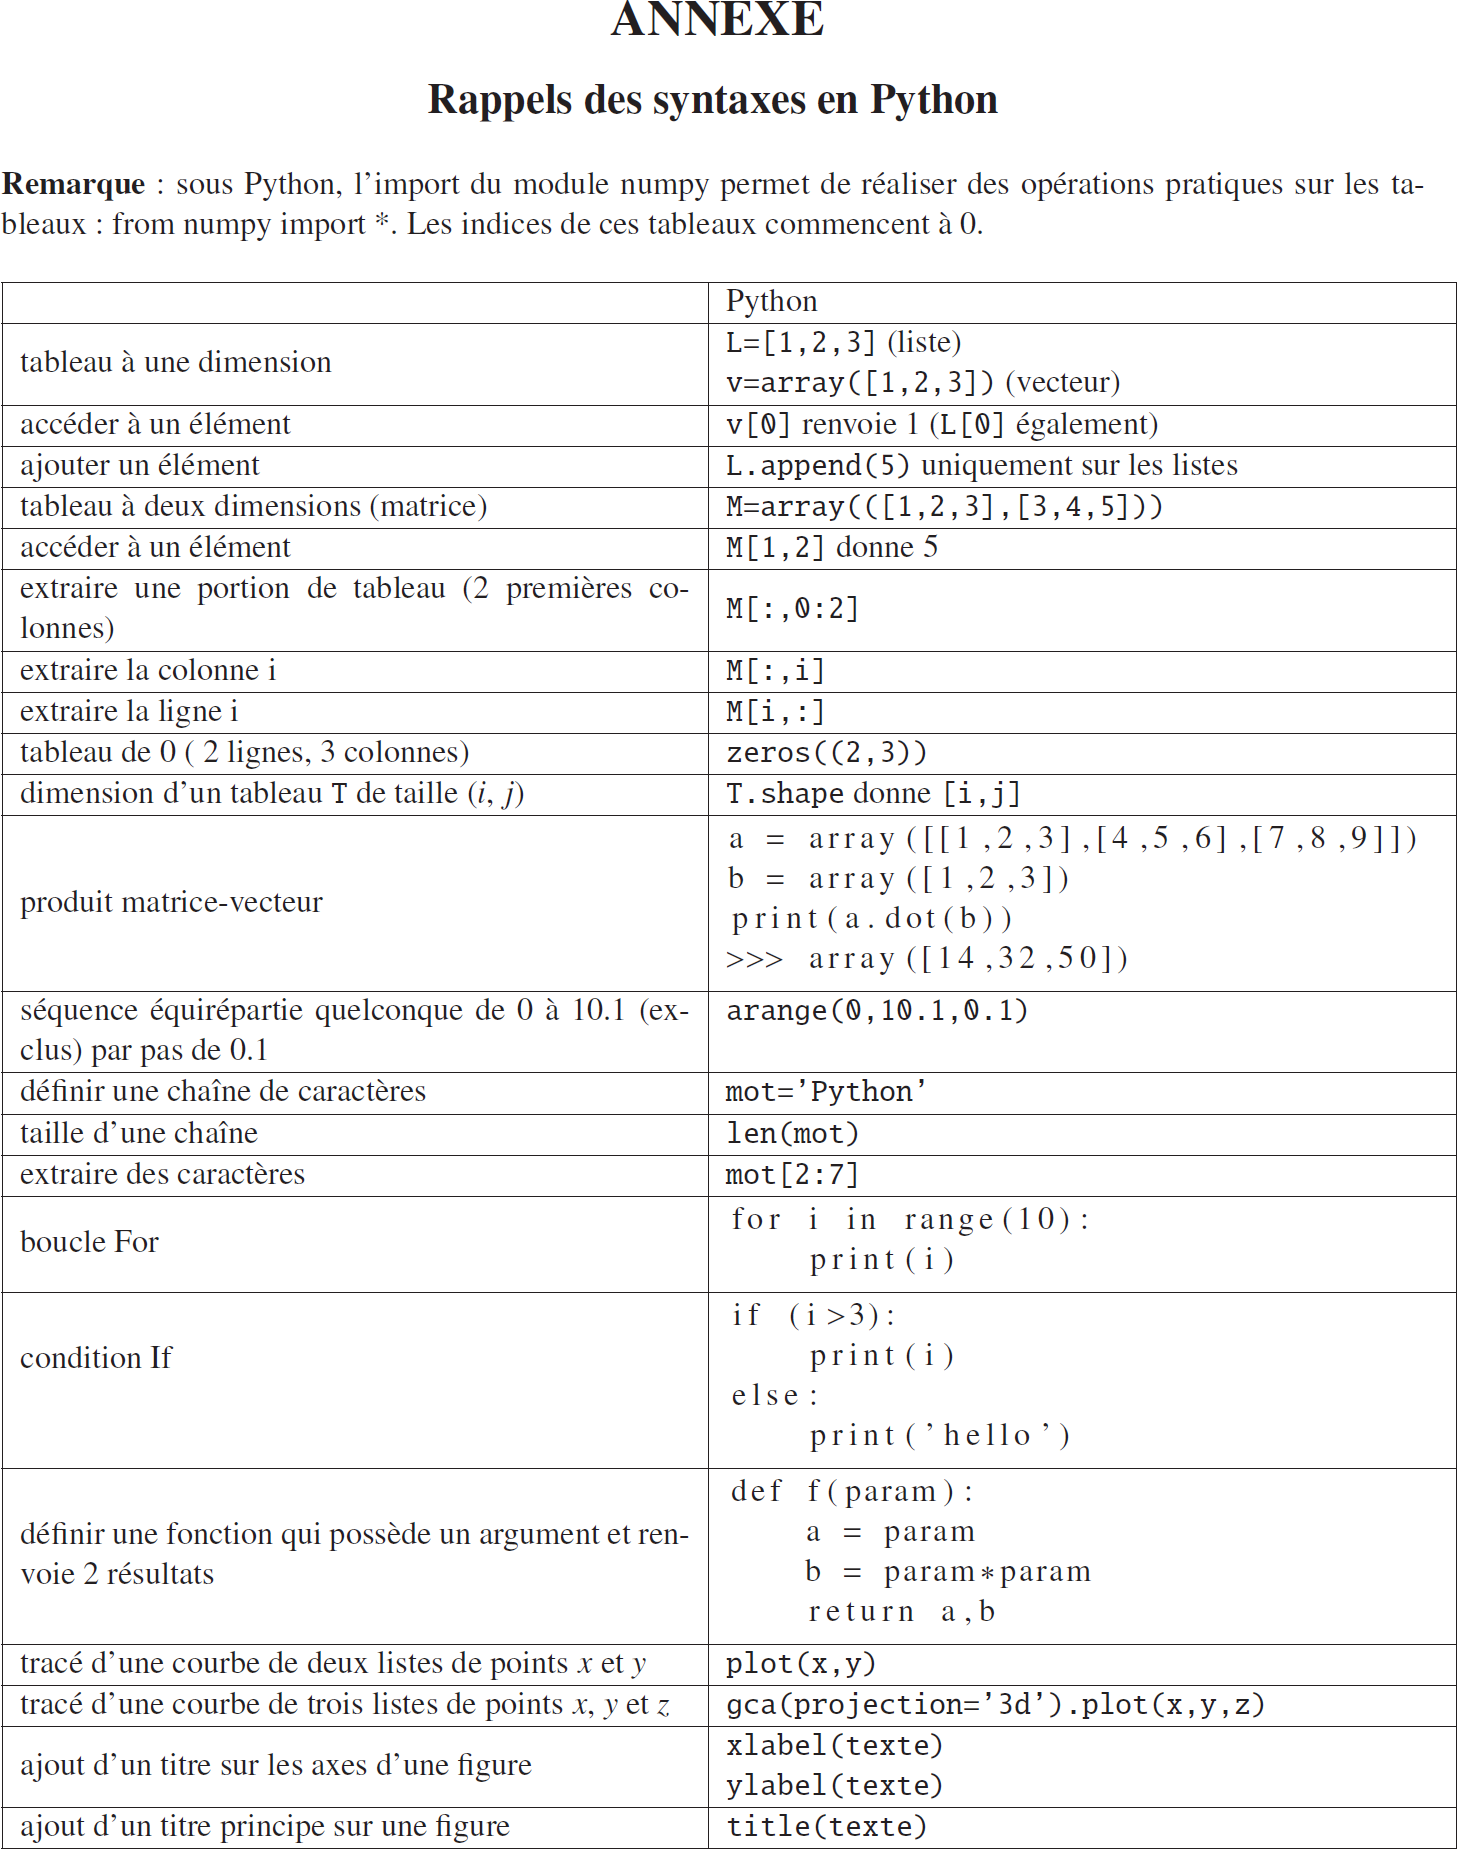
\includegraphics[width=\textwidth]{images/ann_01}
\end{center}
\fi
